\documentclass[
    11pt,     
    a4paper,     
    parskip=full
]{article}

\usepackage[utf8]{inputenc}
\usepackage[T1]{fontenc} 
\usepackage{graphicx}
\usepackage{parskip}

% Titel und Metadaten
\title{\textbf{Werkzeuge für das wissenschaftliche Arbeiten}}
\author{Python for Machine Learning and Data Science}
\date{Abgabe: 15.12.2023}
\renewcommand{\contentsname}{Inhaltsverzeichnis}
\renewcommand{\figurename}{Abbildung}

\begin{document}
    % Titelseite
    \begin{center}
        \Large \textbf{Werkzeuge für das wissenschaftliche Arbeiten}\\[0.1cm]
        \normalsize Python for Machine Learning and Data Science\\[0.1cm]
        \normalsize\centering{Abgabe: 15.12.2023} \\ [0.5cm]
        \hrule % Horizontale Linie
    \end{center}
    
    % Inhaltsverzeichnis
    \tableofcontents 
    \vspace{0.5cm}
    \hrule % Horizontale Linie
    
    % Hauptinhalt
    \section{Projektaufgabe}
        In dieser Aufgabe beschäftigen wir uns mit Objektorientierung in Python.
        Der Fokus liegt auf der Implementierung einer Klasse, dabei nutzen wir insbesondere auch Magic Methods. 
    
        \begin{figure}[h!]
            \centering
            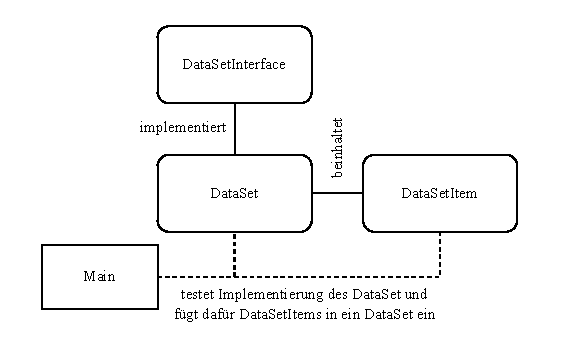
\includegraphics[width=\textwidth]{../diagram/classes_files.pdf}
            \caption{Darstellung der Klassenbeziehungen.}
        \end{figure}
        
        
        \subsection{Einleitung}        
            Ein Datensatz besteht aus mehreren Daten, ein einzelnes Datum wird durch ein Objekt der Klasse \texttt{Data\-Set\-Item} repräsentiert.
            Jedes Datum hat einen Namen (Zeichenkette), eine ID (Zahl) und bel. Inhalt.
            
            Nun sollen mehrere Daten, Objekte vom Typ \texttt{Data\-Set\-Item}, in einem Datensatz zusammengefasst werden.
            Sie haben sich schon auf eine Schnittstelle und die benötigten Operationen, die ein Datensatz unterstützen muss, geeinigt.
            Es gibt eine Klasse \texttt{Data\-Set\-Interface}, die die Schnittstelle definiert und Operationen jedes Datensatzes angibt.
            Bisher fehlt aber noch die Implementierung eines Datensatzes mit allen Operationen.
        
            Implementieren Sie eine Klasse \texttt{Data\-Set} als eine Unterklasse von \texttt{Data\-Set\-Interface}.
            
        
        \subsection{Aufbau}
            Es gibt drei Dateien, \texttt{dataset.py}, \texttt{main.py} und \texttt{implementation.py}$^*$.
            In der \texttt{dataset.py} befinden sich die Klassen \texttt{Data\-Set\-Interface} und \texttt{Data\-Set\-Item},
            in der Datei \texttt{implementation.py} muss die Klasse \texttt{Data\-Set} implementiert werden.
            Die Datei \texttt{main.py} nutzt die Klassen \texttt{Data\-Set} und \texttt{Data\-Set\-Item} aus den jeweiligen Dateien und testet die Schnittstelle und Operationen von \texttt{Data\-Set\-Interface}.
            
        \subsection{Methoden}
            Die folgenden Methoden sollen in der Klasse \texttt{Data\-Set} implementiert werden:
    
            
            \begin{itemize}
                \item \texttt{\_\_setitem\_\_(self, name, id\_content)} 
                \\ Hinzufügen eines Datums.
                \item \texttt{\_\_iadd\_\_(self, item)} 
                \\ Hinzufügen eines \texttt{Data\-Set\-Item}.
                \item \texttt{\_\_delitem\_\_(self, name)} 
                \\ Löschen eines Datums anhand des Namens.
                \item \texttt{\_\_contains\_\_(self, name)} 
                \\ Prüfung, ob ein Datum im Datensatz vorhanden ist.
                \item \texttt{\_\_getitem\_\_(self, name)} 
                \\ Abrufen eines Datums über den Namen.
                \item \texttt{\_\_and\_\_(self, dataset)} 
                \\ Schnittmenge zweier Datensätze als neuen Datensatz zurückgeben.
                \item \texttt{\_\_or\_\_(self, dataset)} 
                \\ Vereinigung zweier Datensätze als neuen Datensatz zurückgeben.
                \item \texttt{\_\_iter\_\_(self)} 
                \\ Iteration über alle Daten.
                \item \texttt{filtered\_iterate(self, filter)} 
                \\ Gefilterte Iteration über einen Datensatz.
                \item \texttt{\_\_len\_\_(self)} 
                \\ Anzahl der Daten abrufen.
            \end{itemize}
    
    \section{Abgabe}
        Programmieren Sie die Klasse \texttt{Data\-Set} in der Datei \texttt{implementation.py} zur Lösung der oben beschrieben Aufgabe im VPL.
        Sie können auch direkt auf Ihrem Computer programmieren, dazu finden Sie alle drei benötigten Dateien zum Download im Moodle.
        
        Das VPL nutzt den gleichen Code, wobei die \texttt{main.py} um weitere Testfälle und Überprüfungen erweitert wurde. 
        Die Überprüfungen dienen dazu sicherzustellen, dass Sie die richtigen Klassen nutzen.
        \\
        \hrule\hfill\\[0.1cm]
        $^*$ Dateien befinden sich im Ordner \texttt{/code/} dieses Git-Repositories.
\end{document}